\chapter{Einleitung}
\label{ch:intro}

% NEU GEFASST am 15.09.2026 nach dem Absatzplan, freigegeben vom Verfasser.
% Befunde B03, E1. Bezug zu BESS und kurativ im Vorspann, Klimaschutzsatz entfallen.
% Alte Fassung, nicht wieder aufnehmen:
%Der anthropogen verursachte Klimawandel erfordert eine grundlegende Transformation des deutschen Energiesystems, für die das Bundes-Klima\-schutz\-gesetz mit der Netto-Treib\-haus\-gas\-neu\-tra\-li\-tät bis zum Jahr 2045 die Zielvorgabe setzt \cite{bundesumweltministerium_bundes-klimaschutzgesetz_2019}.
%Der Anteil erneuerbarer Energien an der Nettostromerzeugung lag im Jahr 2025 bei 58{,}8\,\% \cite{bundesnetzagentur_strommarktdaten_2026}.
%Mit diesem Anteil verändert sich nicht allein die Zusammensetzung der Erzeugung, sondern auch ihre räumliche Verteilung und damit die Transportaufgabe des Übertragungsnetzes.
Der Anteil erneuerbarer Energien an der Nettostromerzeugung lag im Jahr 2025 bei 58{,}8\,\% \cite{bundesnetzagentur_strommarktdaten_2026}.
Mit diesem Anteil verändert sich nicht allein die Zusammensetzung der Erzeugung, sondern auch ihre räumliche Verteilung und damit die Transportaufgabe des Übertragungsnetzes.
% SATZLAENGE am 15.09.2026, Stilregel 17, alte Fassung als Kommentar:
%Die vorliegende Arbeit befasst sich mit einer Antwort auf diese Aufgabe, nämlich der kurativen Systemführung, die das bestehende Netz höher auslastet, und mit \ac{BESS} als dem Akteur, der die dafür nötige Reaktionsfähigkeit bereitstellt.
Die vorliegende Arbeit befasst sich mit einer Antwort auf diese Aufgabe, nämlich der kurativen Systemführung, die das bestehende Netz höher auslastet.
Als Akteur dafür kommen \ac{BESS} in Betracht, die die nötige Reaktionsfähigkeit bereitstellen.

\section{Motivation und Problemstellung}
\label{sec:motivation}

% NEU GEFASST am 15.09.2026 nach dem Absatzplan, freigegeben vom Verfasser.
% Befunde B04 bis B12, E2 bis E6, V12. Achse Nord-Ost nach Sued-West, These mit Doppelpunkt, Redispatch als Kurzform, Ereignisabhaengigkeit benannt.
% Alte Fassung, nicht wieder aufnehmen:
%Die Transportaufgabe des Übertragungsnetzes ist bislang vor allem durch ein geografisches Missverhältnis zwischen den Erzeugungsschwerpunkten der Windkraft im Norden und den industriellen Verbrauchszentren im Süden Deutschlands geprägt, während in der Nähe der Lastzentren steuerbare konventionelle Kraftwerke aus dem Betrieb ausscheiden.
%Der Netzausbau setzt an dieser Achse an und mindert die dort auftretenden Engpässe.
%Mit dem Zubau der Photovoltaik wird das Engpassmuster zugleich vielfältiger, denn eine hohe Einspeisung aus Photovoltaikanlagen führte insbesondere in den Sommermonaten des Jahres 2025 vermehrt zu Ost-West-Lastflüssen \cite{bundesnetzagentur_smard_engpassmanagement_2026}.
%
%Die Architektur des europäischen Strommarktes verstärkt dieses Missverhältnis.
%Im Selbst\-dispatch-Modell bestimmen die Fahrplanverantwortlichen die Erzeugungs- und Verbrauchsfahrpläne sowie den Einsatz ihrer Anlagen selbst \cite{europaisches_parlament_und_rat_der_eu_verordnung_2019}.
%Der deutsche Strommarkt folgt diesem Modell.
%Maßgeblich für den Einsatz ist damit das Preissignal des Marktes und nicht der Zustand des Netzes.
%Innerhalb einer einheitlichen Gebotszone bildet der Börsenpreis die physikalische Belastung der Übertragungswege jedoch nicht ab, sodass marktoptimale Fahrpläne systematisch Leistungsflüsse erzeugen können, die das Netz nicht aufnehmen kann.
%Der \ac{ÜNB} kann auf die Fahrplanbildung nicht einwirken und die entstehende Netzüberlastung deshalb erst nachgelagert korrigieren.
%Die Höhe des Engpassmanagementbedarfs folgt damit nicht allein aus der Netzsituation, sondern auch aus der Entkopplung von marktlicher Fahrplanbildung und physikalischer Netzrestriktion.
%
%Wie hoch der daraus folgende Eingriffsbedarf ausfällt, zeigen die Zahlen des Netzengpassmanagements.
%Abbildung~\ref{fig:redispatch_jahresbedarf} stellt das jährliche Maßnahmenvolumen des Netzengpassmanagements dar, das die Reduzierung der Einspeisung und die zu deren Ausgleich erforderliche Erhöhung umfasst.
%Mit 30{,}4\,\si{TWh} lag es im Jahr 2025 nahezu auf dem Wert des Vorjahres.
%Die vorläufigen Gesamtkosten stiegen dagegen um knapp vier Prozent auf rund 3{,}1\,Mrd.\,Euro.
%Die Jahressummen verdecken dabei eine ausgeprägte Ereignisabhängigkeit.
%Die monatlichen Gesamtkosten variierten seit Juli 2022 zwischen rund 123\,Mio.\,Euro im Juni 2023 und rund 485\,Mio.\,Euro im Dezember 2024.
%Auf diesen Monat entfielen rund 16\,\% der Jahresgesamtkosten 2024 \cite{bundesnetzagentur_mengen_nodate}.
%Ausschlaggebend für diesen Ausreißer war eine Windfront im Dezember 2024 \cite{bundesnetzagentur_smard_engpassmanagement_2026}.
% SATZLAENGE am 15.09.2026, Stilregel 17, alte Fassung als Kommentar:
%Die Transportaufgabe des Übertragungsnetzes ist durch ein geografisches Missverhältnis geprägt, denn die Windkraft speist vor allem im Norden und Osten Deutschlands ein, die Lastzentren liegen im Süden und Westen, und in deren Nähe scheiden steuerbare konventionelle Kraftwerke aus dem Betrieb aus.
Die Transportaufgabe des Übertragungsnetzes ist durch ein geografisches Missverhältnis geprägt: Die Windkraft speist vor allem im Norden und Osten Deutschlands ein, die Lastzentren liegen im Süden und Westen.
In der Nähe der Lastzentren scheiden zudem steuerbare konventionelle Kraftwerke aus dem Betrieb aus.
Während der Netzausbau an dieser Achse von Nordosten nach Südwesten ansetzt, wird das Engpassmuster mit dem Zubau der Photovoltaik zugleich vielfältiger, denn eine hohe Einspeisung aus Photovoltaikanlagen führte in den Sommermonaten des Jahres 2025 vermehrt zu Ost-West-Lastflüssen \cite{bundesnetzagentur_smard_engpassmanagement_2026}.
Die Transportaufgabe ist damit nicht auf eine Richtung festgelegt.

Das Marktdesign des europäischen Binnenmarkts, dem der deutsche Strommarkt folgt, verstärkt dieses Missverhältnis: Im Selbst\-dispatch-Modell bestimmen die Fahrplanverantwortlichen die Erzeugungs- und Verbrauchsfahrpläne sowie den Einsatz ihrer Anlagen selbst \cite{europaisches_parlament_und_rat_der_eu_verordnung_2019}.
Maßgeblich für den Einsatz ist damit das Preissignal des Marktes und nicht der Zustand des Netzes.
Innerhalb der einheitlichen Gebotszone, in der für ganz Deutschland ein Börsenpreis gilt, bildet dieser Preis die Belastung der Übertragungswege nicht ab, sodass marktoptimale Fahrpläne regelmäßig Leistungsflüsse erzeugen, die das Netz nicht aufnehmen kann.
Der \ac{ÜNB} kann mit den Fahrplänen, die die Akteure ihm melden, die Leistungsflüsse im Netz nur vorhersagen und eine drohende Überlastung anschließend durch Redispatch beheben, also durch die angeordnete Anpassung der Einspeisung einzelner Anlagen.
Der Redispatchbedarf ist damit nicht allein eine Folge des Netzzustands, sondern auch eine Folge des Marktdesigns.

Wie hoch dieser Bedarf ausfällt, zeigt Abbildung~\ref{fig:redispatch_jahresbedarf} mit dem jährlichen Redispatchvolumen, also der reduzierten und der zu ihrem Ausgleich erhöhten Einspeisung.
Mit 30{,}4\,\si{TWh} lag das Redispatchvolumen im Jahr 2025 nahezu auf dem Wert des Vorjahres, während die vorläufigen Gesamtkosten um knapp vier Prozent auf rund 3{,}1\,Mrd.\,Euro stiegen.
Die Jahressummen verdecken dabei, wie stark einzelne Wetterlagen die Kosten prägen: Die monatlichen Gesamtkosten schwankten seit Juli 2022 zwischen rund 123\,Mio.\,Euro im Juni 2023 und rund 485\,Mio.\,Euro im Dezember 2024 \cite{bundesnetzagentur_mengen_nodate}.
Auf den Dezember 2024, geprägt von einer Windfront, entfielen rund 16\,\% der Jahresgesamtkosten 2024, sodass wenige Tage über die Kosten eines Jahres mitentscheiden \cite{bundesnetzagentur_smard_engpassmanagement_2026}.

\begin{figure}[htbp]
    \centering
% GROESSENANGABE ERGAENZT am 12.09.2026 nach der Anweisung des Verfassers.
% Sie aendert den Satz nicht, die Datei ist genau textbreit.
    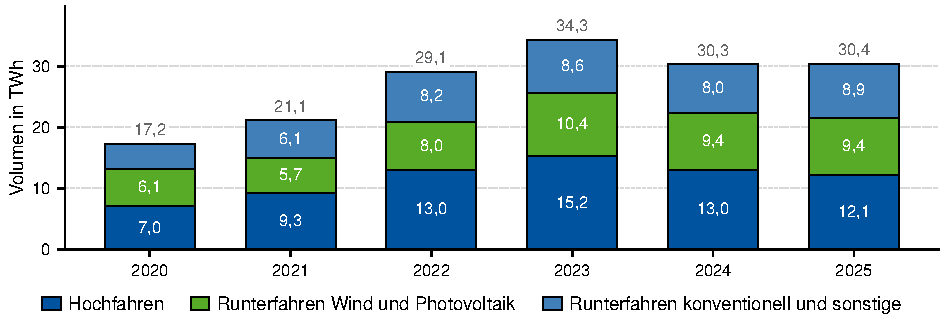
\includegraphics[width=\textwidth]{figures/chapter_1/redispatch_jahresbedarf_2020_2025.pdf}
    \caption{Jährliches Maßnahmenvolumen des Netzengpassmanagements der Jahre 2020 bis 2025, aufgeteilt nach hoch- und heruntergeregelter Energie. Alle Maßnahmen sind einer der beiden Richtungen zugeordnet. Auf Basis von \cite{bundesnetzagentur_mengen_nodate}.}
    \label{fig:redispatch_jahresbedarf}
\end{figure}

% NEU GEFASST am 15.09.2026 nach dem Absatzplan, freigegeben vom Verfasser.
% Befunde B13 bis B17, E7, E8. These und Begruendung verbunden, 13 TWh einmal, Konsequenz fuer das Instrument ergaenzt.
% Alte Fassung, nicht wieder aufnehmen:
%Für die vorliegende Arbeit ist bedeutsam, dass es sich bei diesem Bedarf nicht um ein Übergangsphänomen handelt, das mit dem Netzausbau vollständig verschwindet.
%Der aktuelle \ac{NEP} weist im Referenzszenario~B, das sich an den Zielvorgaben des Bundes-Klima\-schutz\-gesetzes orientiert, bei einem ausgewiesenen Investitionsbedarf von rund 392\,Mrd.\,Euro noch für das Zieljahr 2045 einen strukturellen Engpassmanagementbedarf von rund 13\,\si{TWh} aus.
%Abbildung~\ref{fig:engpassmanagement_nep} stellt diesen Bedarf den Zieljahren 2032, 2037 und 2045 gegenüber.
%Der Bedarf sinkt bis zum Zieljahr 2037 auf 5{,}4 bis 8{,}6\,\si{TWh} und steigt bis 2045 in allen drei Szenarien wieder auf 11{,}1 bis 13{,}0\,\si{TWh}.
%Der ausgewiesene Restbedarf folgt aus der Zielsetzung des Verfahrens.
%Der \ac{NEP} bestimmt den Netzausbau als Minimalkostenkombination aus Netzausbauinvestitionen und verbleibenden Engpassmanagementkosten \cite{bundesnetzagentur_netzentwicklungsplan_2026}, führt den Ausbau also nur so weit, wie er die Engpassmanagementkosten um mehr senkt, als er selbst verursacht.
%Ein verbleibendes Eingriffsvolumen ist damit Bestandteil des ermittelten Zielzustands und nicht Ausdruck eines unvollständigen Ausbaustands.
%Seine Deckung fällt damit Instrumenten jenseits des Netzausbaus zu.
%
%Die dargestellten Zahlen und das beschriebene Engpassmuster zeigen dabei zwei Eigenschaften des Bedarfs, die für die Wahl des Instruments bedeutsam sind.
%Zum einen ist der Bedarf ereignisabhängig, denn Volumen und Kosten entwickeln sich nicht proportional zueinander, und einzelne Wetterlagen prägen den Kostenverlauf eines Jahres stärker als die Jahresmenge.
%Zum anderen verschiebt sich das räumliche Engpassmuster mit der jeweils vorherrschenden Erzeugungssituation.
Der Redispatchbedarf ist kein Übergangsphänomen, das mit dem Netzausbau verschwindet, denn der aktuelle \ac{NEP} weist im Szenario~B, einem von drei Szenarien, bei einem Investitionsbedarf von rund 392\,Mrd.\,Euro noch für das Zieljahr 2045 einen strukturellen Engpassmanagementbedarf von rund 13\,\si{TWh} aus.
Abbildung~\ref{fig:engpassmanagement_nep} zeigt den Verlauf: Der Bedarf sinkt bis zum Zieljahr 2037 auf 5{,}4 bis 8{,}6\,\si{TWh} und steigt bis 2045 in allen drei Szenarien wieder auf 11{,}1 bis 13{,}0\,\si{TWh}.
Der Restbedarf für das Jahr 2045 folgt aus der Zielsetzung des Verfahrens, denn der \ac{NEP} bestimmt den Netzausbau als Minimalkostenkombination aus Ausbauinvestitionen und verbleibenden Engpassmanagementkosten und führt den Ausbau nur so weit, wie die eingesparten Engpassmanagementkosten die Ausbaukosten übersteigen \cite{bundesnetzagentur_netzentwicklungsplan_2026}.
Ein verbleibender Engpassmanagementbedarf gehört damit zum ermittelten Zielzustand und fällt Instrumenten jenseits des Netzausbaus zu.

Die dargestellten Zahlen zeigen zwei Eigenschaften des Engpassmanagementbedarfs, die für die Wahl eines solchen Instruments bedeutsam sind.
Der Bedarf ist ereignisabhängig, denn einzelne Wetterlagen prägen den Kostenverlauf eines Jahres stärker als die Jahresmenge.
Zugleich wandert das Engpassmuster räumlich, denn es verschiebt sich mit der jeweils vorherrschenden Erzeugungssituation.
% EIGENE ABLEITUNG, vom Verfasser zu pruefen, Absatzplan 1.1 Absatz 5 vom 15.09.2026.
Ein Instrument für den Engpassmanagementbedarf muss deshalb im Ereignisfall wirken, ohne dauerhaft Eingriffe zu verursachen, und an wechselnden Orten verfügbar sein.

\begin{figure}[htbp]
    \centering
% GROESSENANGABE ERGAENZT am 12.09.2026 nach der Anweisung des Verfassers.
% Sie aendert den Satz nicht, die Datei ist genau textbreit.
    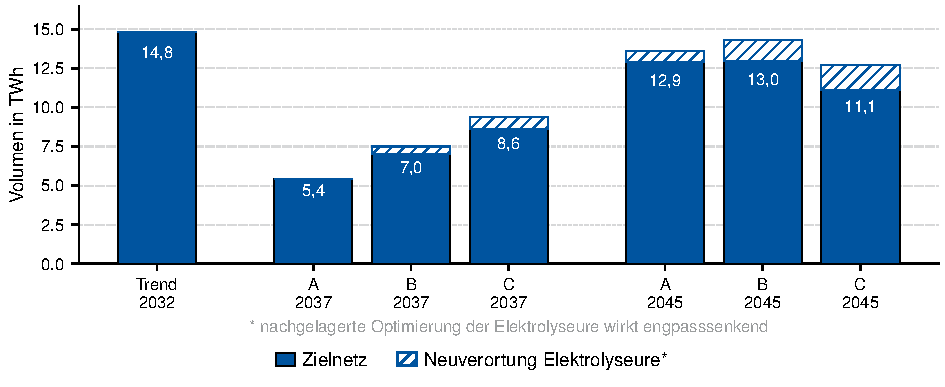
\includegraphics[width=\textwidth]{figures/chapter_1/engpassmanagement_nep.pdf}
    \caption{Engpassmanagementbedarf der Zieljahre 2032, 2037 und 2045 nach Netzentwicklungsplan. Auf Basis von \cite{bundesnetzagentur_netzentwicklungsplan_2026}.}
    \label{fig:engpassmanagement_nep}
\end{figure}

% NEU GEFASST am 15.09.2026 nach dem Absatzplan, freigegeben vom Verfasser.
% Befunde B18 bis B23, E9, E10, V13. Reihenfolge neu, praeventiv vor der zeitlichen Luecke, Reaktion des UENB auf spaete Zustaende ergaenzt, kurativ nicht als einzige Antwort.
% Alte Fassung, nicht wieder aufnehmen:
%Neben dem Volumen verändert sich die zeitliche Struktur der Engpässe.
%Die präventive Betriebsplanung setzt voraus, dass die Netzbelastung des Erfüllungszeitpunkts vorab hinreichend genau bekannt ist, denn nur dann lässt sich die (N-1)-Sicherheit rechtzeitig herstellen.
%Mit der Zunahme kurzfristig agierender Flexibilität wird diese Voraussetzung schwerer einzuhalten.
%Der kontinuierliche Intraday-Handel hält die Fahrplanbildung bis wenige Minuten vor Lieferbeginn offen, und Anlagen mit kurzen Reaktionszeiten können dieses späte Handelsfenster nutzen \cite{innosys_2030_gesamtverbund_innovationen_2021, mahgoub_wie_2025}.
%Besonders für Batteriespeicher, im Folgenden als \ac{BESS} bezeichnet, liefert die Nachjustierung in diesem Fenster einen eigenständigen Wertbeitrag \cite{hornek_value_2025}.
%Der \ac{ÜNB} prüft die Netzbelastung dabei in Vorschauprozessen am Vortag und im Verlauf des Erfüllungstages sowie in einer laufenden Netzsicherheitsrechnung auf der aktuellen Netzsituation \cite{leeuwen_integration_2020}.
%Die Vorschauprozesse enden jedoch vor dem Erfüllungszeitpunkt, sodass Fahrplanänderungen aus dem danach verbleibenden Handelsfenster in ihnen nicht mehr enthalten sind.
%Dem Marktteilnehmer wiederum zeigt der zonale Preis die Netzbelastung nicht an.
%Verändern sich die Leistungsflüsse nach der letzten Netzsicherheitsrechnung vor dem Erfüllungszeitpunkt, kann ein Zustand entstehen, der nicht mehr (N-1)-sicher ist, weil sich eine präventive Gegenmaßnahme nicht mehr rechtzeitig disponieren lässt.
%
%Die Versorgungssicherheit im operativen Betrieb der \ac{ÜNB} beruht vorrangig auf präventiver Systemführung, bei der Betriebsmittel unterhalb ihrer dauerhaften physikalischen Kapazitätsgrenze betrieben werden.
%Die so freigehaltene Sicherheitsmarge hält das System im Fehlerfall stabil.
%Dabei bleibt eine physikalische Reserve systematisch ungenutzt, denn Betriebsmittel lassen sich kurzfristig höher belasten, als im Dauerbetrieb zulässig ist.
%Die kurative Systemführung vermeidet Engpässe nicht im Voraus, sondern behebt sie nach ihrem Eintreten durch gezielte Gegenmaßnahmen.
%Sie nutzt dafür diese Reserve und ermöglicht damit eine effizientere Nutzung des bestehenden Netzes.
%Sie setzt an demselben Eingriffsbedarf an, den die vorangehenden Absätze beziffert haben, denn eine Vorauslastung, die bisher durch eine präventive Maßnahme begrenzt werden musste, wird zulässig.
%Weil ein Abruf nur im Fehlerfall erfolgt, fällt zudem weniger Maßnahmenvolumen an als bei einer Vorsorge, die für jede Ausfallvariante im Voraus getroffen wird.
%Sie liegt zugleich hinter der letzten Netzsicherheitsrechnung, sodass ihr die zuvor beschriebene zeitliche Lücke nicht entgegensteht.
%Voraussetzung dafür ist allerdings ein Akteur, dessen Technologie innerhalb des verbleibenden kurzen Zeitfensters zuverlässig reagiert und dessen Stellpotenzial nicht durch die eigene marktliche Fahrplanbildung aufgebraucht wurde.
%Als vergleichsweise neuer Akteur im Stromnetz erscheinen \ac{BESS} dafür auf den ersten Blick gut geeignet, was Abschnitt \ref{sec:actor_comparison} eingehender prüft.
Wie ein Instrument im Ereignisfall wirken kann, hängt davon ab, wie der \ac{ÜNB} Engpässe heute beherrscht: Die Versorgungssicherheit im operativen Betrieb beruht auf präventiver Systemführung.
Jedes Betriebsmittel hat eine Belastung, die es dauerhaft führen kann.
Die präventive Systemführung plant den Einsatz so, dass auch nach dem Ausfall eines Betriebsmittels kein anderes über die Dauergrenze belastet wird, was als (N-1)-Kriterium bezeichnet wird.
Die präventive Systemführung hält die Belastung deshalb im Normalbetrieb um eine Marge unter der Dauergrenze, und das Freihalten dieser Marge ist der Eingriff, der als Redispatch anfällt.
Betriebsmittel vertragen kurzzeitig jedoch mehr, als im Dauerbetrieb zulässig ist, sodass bei der präventiven Systemführung eine physikalische Reserve ungenutzt bleibt \cite{innosys_2030_gesamtverbund_innovationen_2021}.
Die ungenutzte Reserve ist der Ansatzpunkt der kurativen Systemführung.

Die präventive Planung setzt zudem voraus, dass die Netzbelastung des Erfüllungszeitpunkts vorab hinreichend genau bekannt ist, und damit tritt zu Volumen und Ort als dritte Eigenschaft der Zeitpunkt, zu dem ein Engpass erkennbar wird.
Der \ac{ÜNB} prüft die Netzbelastung in Vorschauprozessen am Vortag und im Verlauf des Erfüllungstages \cite{leeuwen_integration_2020}, und zwischen der letzten Vorschaurechnung und dem Lieferbeginn bleibt ein Handelsfenster offen, das für den Handel innerhalb einer Regelzone, also des Netzgebiets eines \ac{ÜNB}, erst fünf Minuten vor Lieferung schließt.
Fahrplanänderungen nach der letzten Vorschaurechnung gehen in keine Rechnung mehr ein, und gerade Anlagen mit kurzen Reaktionszeiten wie \ac{BESS} handeln in diesem späten Fenster, weil die Nachjustierung dort einen eigenen Wertbeitrag liefert \cite{mahgoub_wie_2025, hornek_value_2025}.
% SETZUNG nach V13, entschieden vom Verfasser am 14.09.2026. Beleg in
% leeuwen_integration_2020 zu suchen, bis dahin ohne Zitat.
Entsteht durch solche späten Änderungen ein Zustand, der nicht mehr (N-1)-sicher ist, erkennt ihn der \ac{ÜNB} in der laufenden Netzsicherheitsrechnung auf der aktuellen Netzsituation.
% SATZLAENGE am 15.09.2026, Stilregel 17, alte Fassung als Kommentar:
%Der \ac{ÜNB} behebt einen solchen Zustand mit Schaltmaßnahmen, Phasenschiebern und kurzfristigem Redispatch derjenigen Anlagen, die noch reagieren können, sodass das Netz sicher bleibt, der Eingriff aber teurer wird und der Kreis geeigneter Anlagen kleiner ist als in der Vorplanung.
Der \ac{ÜNB} behebt einen solchen Zustand mit Schaltmaßnahmen, Phasenschiebern und kurzfristigem Redispatch derjenigen Anlagen, die noch reagieren können.
Das Netz bleibt damit sicher.
Der Eingriff wird aber teurer als in der Vorplanung, weil der Kreis geeigneter Anlagen kleiner ist.

Die kurative Systemführung vermeidet Engpässe nicht im Voraus, sondern behebt sie nach ihrem Eintreten durch gezielte Gegenmaßnahmen und nutzt dafür die kurzzeitige Überlastbarkeit der Betriebsmittel \cite{innosys_2030_gesamtverbund_innovationen_2021}.
% SATZLAENGE am 15.09.2026, Stilregel 17, alte Fassung als Kommentar:
%Damit wird eine Vorauslastung zulässig, die bisher durch eine präventive Maßnahme begrenzt werden musste, sodass ein Teil des Redispatch entfällt, der heute allein dazu dient, die Marge freizuhalten.
Damit wird eine Vorauslastung zulässig, die bisher durch eine präventive Maßnahme begrenzt werden musste.
Ein Teil des Redispatch entfällt deshalb, nämlich der Teil, der heute allein dazu dient, die Marge freizuhalten.
Der Redispatch selbst entfällt damit nicht, denn nach einem Abruf stellt ein Redispatch den (N-1)-sicheren Zustand wieder her.
Weil ein Abruf nur im Fehlerfall erfolgt, fällt zudem weniger Maßnahmenvolumen an als bei einer Vorsorge, die für jeden möglichen Ausfall im Voraus getroffen wird.
Die zeitliche Lücke zwischen der letzten Vorschaurechnung und dem Lieferbeginn besteht auch für die kurative Systemführung, denn die kurative Maßnahme wird ebenfalls vorab eingeplant, und ob sie sich in dieser Lücke noch anpassen lässt, hängt vom jeweiligen Konzept ab.
Voraussetzung eines kurativen Eingriffs sind allerdings Akteure in Bereitschaft, deren Anlagen innerhalb weniger Minuten zuverlässig reagieren und deren Stellpotenzial, also die Leistung, um die sie ihren Betriebspunkt noch verändern können, nicht durch die eigene marktliche Fahrplanbildung aufgebraucht ist.
\ac{BESS} erscheinen als solche Akteure geeignet, wie in Abschnitt~\ref{sec:actor_comparison} dargestellt.

\section{Zielsetzung und Vorgehensweise}
\label{sec:research_questions}
\label{sec:structure}

% NEU GEFASST am 15.09.2026 nach dem Absatzplan im Sammelmodus, Befunde
% B24 bis B39, E11 bis E14, P1, P6, P8, V2, V12. Definitionen von kurativer
% Vorhaltung, kurativer Reservierung, Bindung, Bindungsdauer und Reaktionszeit,
% Kapitelueberblick mit handelnden Subjekten. Alte Fassung, nicht wieder aufnehmen:
%Die vorliegende Arbeit verfolgt das Ziel, einen Marktmechanismus für die kurative Vorhaltung zu entwerfen und den kurativen Reservierungspreis zu bestimmen.
%Das Verbundprojekt InnoSys~2030 hat das Potenzial der kurativen Systemführung für den deutschen Übertragungsnetzbetrieb untersucht und die dafür in Betracht kommenden Maßnahmen systematisiert \cite{innosys_2030_gesamtverbund_innovationen_2021}.
%Die kurative Vorhaltung ist dabei selbst eine Systemdienstleistung und gehört innerhalb der üblichen Einteilung zur Betriebsführung, zu der auch das Engpassmanagement zählt.
%Den Redispatch, also die vom \ac{ÜNB} angeordnete Anpassung der Einspeisung einzelner Anlagen zur Behebung eines Engpasses, ersetzt sie nicht, sondern ergänzt ihn um einen Eingriff nach dem Eintritt des Fehlerfalles.
%Für ihre Beschaffung ist die marktliche Form vorrangig, weil sie den kostenoptimalen Betrieb des Systems unterstützt \cite{europaisches_parlament_und_rat_der_eu_verordnung_2019}.
%Da der Anlagenbetreiber im Selbst\-dispatch-Modell über den Einsatz seiner Anlage entscheidet, lässt sich kurative Verfügbarkeit über einen Anreiz herbeiführen.
%Dieser Anreiz muss aus einer Vergütung folgen, und innerhalb der Systemdienstleistungen bestehen dafür mehrere Vergütungslogiken.
%Die Frequenzhaltung wird über die Regelleistungsmärkte beschafft, die vorgehaltene Leistung im Wettbewerb kaufen und damit die Bereitstellung und nicht allein den Abruf vergüten \cite{ubertragungsnetzbetreiber_deutschland_praqualifikationsverfahren_2024}.
%Das Engpassmanagement folgt demgegenüber keiner Vorhaltelogik, denn der Redispatch wird nach §\,13a \ac{EnWG} angeordnet und über einen finanziellen Ausgleich für den durchgeführten Eingriff entschädigt \cite{bundesministerium_der_justiz_energiewirtschaftsgesetz_2025, bundesnetzagentur_festlegung_2024}.
%Ob eine dieser beiden Logiken den erforderlichen Anreiz für die kurative Vorhaltung setzt, ist damit zu klären.

%Der Betrachtungsrahmen ist ein 2030-Szenario mit hohem Anteil erneuerbarer Energien, fortbestehenden Netzausbaurückständen und gestiegener installierter Speicherkapazität.
%Die Arbeit rechnet gleichwohl mit den Preiszeitreihen des Jahres 2025.
%Eine Preisprognose für das Zieljahr wäre nicht überprüfbar und würde das Ergebnis mit einer zweiten Unsicherheit belasten, während beobachtete Preise nachvollziehbar sind und die für das Szenario maßgebliche Volatilität bereits aufweisen.
%Bestimmt wird daraus der kurative Reservierungspreis, also der Betrag, den ein Anlagenbetreiber für die Bindung mindestens fordern muss, um gegenüber seinen übrigen Vermarktungswegen indifferent zu sein.
%Er bemisst die entgangenen Erlösmöglichkeiten und ist damit eine Eigenschaft der Anlage und ihres Umfelds.
%Das Entlastungspotenzial der kurativen Systemführung schätzt die Arbeit nicht ab, sie bestimmt allein den Preis ihrer Vorhaltung.
%Wie hoch er ausfällt, folgt aus der Ausgestaltung des Produkts, also aus der Bindungsdauer, der geforderten Reaktionszeit und der vorzuhaltenden Leistung.
%Auf den Preis, der sich am Markt einstellt, wirken zusätzlich die Präqualifikationsanforderungen, die Pönale bei Nichtlieferung, die Liquidität am jeweiligen Netzknoten und die Zahl der dort geeigneten Anbieter.
%Zu klären sind dazu drei Teilfragen, nämlich welche Anforderungen die kurative Systemführung an ein Marktprodukt stellt, wie sich eine Vorhalteverpflichtung auf Fahrplan und Erlöse einer Anlage auswirkt und wie sich der daraus folgende Reservierungspreis in die bestehenden Vergütungslogiken für Systemdienstleistungen einordnet.

%Kapitel~\ref{ch:state_of_the_art} behandelt die kurative Systemführung und die für sie in Betracht kommenden Technologien, stellt den Marktrahmen mit seinen Dispatchmodellen, Marktzeithorizonten und Systemdienstleistungen dar und untersucht die Vergütungslogiken des Engpassmanagements und der Regelleistung.
%Es begründet die Wahl der \ac{BESS} als kurativen Akteur und prüft, welche der bestehenden Vergütungslogiken auf die kurative Vorhaltung passt.
% NACHZUZIEHEN nach der Aufloesung von 3.1.3 am 11.09.2026. Kapitel 3 ordnet
% die Marktdesignansaetze jetzt hinter dem Anforderungskatalog ein, und der
% Forschungsbedarf steht nach dem Produktentwurf am Anfang von Abschnitt 3.2.
% Die Reihenfolge dieses und des folgenden Satzes trifft damit nicht mehr zu.
% Die Neufassung waehlt der Verfasser.
% SATZPAAR ERSETZT am 11.09.2026, Fassung C, gewaehlt vom Verfasser. Die
% Reihenfolge folgt jetzt dem Aufbau von Kapitel 3, die Marktdesignansaetze
% werden eingeordnet statt abgeglichen, das Produkt heisst kurative
% Reservierung, und der Forschungsbedarf entfaellt im Ueberblick, weil der
% erste Satz von Abschnitt 1.2 das Ziel der Arbeit nennt. Alte Fassung, nicht
% wieder aufnehmen:
%   Kapitel~\ref{ch:design_model} leitet die Anforderungen an einen kurativen Marktmechanismus ab, gleicht sie gegen bestehende Marktdesignansätze ab und benennt den Forschungsbedarf.
%   Darauf aufbauend entwirft es das kurative Marktprodukt, legt die Systemgrenzen der Untersuchung fest und formuliert die Fahrplanbildung des Speichers als gemischt-ganz\-zahliges lineares Optimierungsproblem.
% GEKUERZT am 14.09.2026, entschieden vom Verfasser. Die Einordnung der
% Marktdesignansaetze ist in 3.1.1 gestrichen, der Ueberblick kuendigte sie
% sonst weiter an. Alte Fassung:
%Kapitel~\ref{ch:design_model} leitet die Anforderungen an einen kurativen Marktmechanismus ab, ordnet bestehende Marktdesignansätze daran ein und entwirft die kurative Reservierung als Produkt.
%Kapitel~\ref{ch:design_model} leitet die Anforderungen an einen kurativen Marktmechanismus ab und entwirft aus ihnen die kurative Reservierung als Produkt.
%Darauf aufbauend legt es die Systemgrenzen der Untersuchung fest und formuliert die Fahrplanbildung des Speichers als gemischt-ganz\-zahliges lineares Optimierungsproblem.
%Es beschreibt die verwendeten Eingangsdaten, begründet, weshalb sich die geltende Bemessungslogik für entgangene Erlösmöglichkeiten nicht in dieses Modell überführen lässt, und verifiziert die Implementierung gegen einen veröffentlichten Erlösindex für \ac{BESS}.
%Kapitel~\ref{ch:results} untersucht, wie sich eine kurative Vorhaltepflicht in den Betrieb eines Marktteilnehmers einfügt.
%Es stellt den Fahrplan, den Ladezustandsverlauf und die Erlöse unter Bindung dar, variiert anschließend die Produkt- und Anlagenparameter und bestimmt daraus den kurativen Reservierungspreis.
%Kapitel~\ref{ch:discussion} ordnet dieses Ergebnis in die bestehenden Vergütungslogiken für Systemdienstleistungen ein, gleicht das entworfene Produkt gegen die Anforderungen ab und würdigt die Modellannahmen kritisch.
%Kapitel~\ref{ch:conc} fasst die Ergebnisse entlang der Forschungsfragen zusammen und benennt weiteren Forschungsbedarf.
Die vorliegende Arbeit verfolgt das Ziel, einen kurativen Marktmechanismus zu entwerfen und den kurativen Reservierungspreis zu bestimmen.
Kurative Vorhaltung bezeichnet dabei das Bereithalten von Leistung und, bei Speichern, von Ladezustand für einen Abruf nach dem Fehler.
Der kurative Marktmechanismus ist das Verfahren, mit dem der \ac{ÜNB} diese Vorhaltung marktlich beschafft, und die kurative Reservierung ist das Produkt, das er dabei ausschreibt, bezuschlagt und vergütet.
% VORGABE DES VERFASSERS am 15.09.2026, Zweck des Mechanismus.
Der Mechanismus wird entworfen, um die Einflüsse zu erkennen, die am Markt auf den Preis einer solchen Reservierung wirken, und nicht, um ein Marktdesign mit prognostizierten Preisen festzulegen.
% VERSCHOBEN am 15.09.2026 nach 1.1 Absatz 8, entschieden vom Verfasser, der Satz wirkte hier fehl am Platz. Alte Fassung:
%Die kurative Systemführung verringert den präventiven Redispatch, ersetzt ihn aber nicht, denn nach einem Abruf stellt ein Redispatch den (N-1)-sicheren Zustand wieder her.
% SATZLAENGE am 15.09.2026, Stilregel 17, alte Fassung als Kommentar:
%Ein Marktmechanismus ist nötig, weil sich die Bereitschaft der Akteure, die Abschnitt~\ref{sec:motivation} als Voraussetzung nennt, im Selbst\-dispatch-Modell nicht anordnen lässt: Der Anlagenbetreiber entscheidet über den Einsatz seiner Anlage selbst, und kurative Verfügbarkeit entsteht deshalb nur über eine Vergütung.
Abschnitt~\ref{sec:motivation} nennt die Bereitschaft der Akteure als Voraussetzung.
Ein Marktmechanismus ist nötig, weil sich die Bereitschaft der Akteure im Selbst\-dispatch-Modell nicht anordnen lässt: Der Anlagenbetreiber entscheidet über den Einsatz seiner Anlage selbst.
Kurative Verfügbarkeit entsteht deshalb nur über eine Vergütung.
Für Systemdienstleistungen bestehen dafür zwei Logiken: Die Regelleistungsmärkte, auf denen die \ac{ÜNB} Leistung für die Frequenzhaltung beschaffen, vergüten die Bereitstellung vorgehaltener Leistung \cite{ubertragungsnetzbetreiber_deutschland_praqualifikationsverfahren_2024}, das Engpassmanagement vergütet nach §\,13a \ac{EnWG} allein den durchgeführten Eingriff \cite{bundesministerium_der_justiz_energiewirtschaftsgesetz_2025, bundesnetzagentur_festlegung_2024}.
Ob die Vergütung der Bereitstellung oder die Vergütung des Eingriffs den erforderlichen Anreiz für die kurative Vorhaltung setzt, ist damit zu klären.

Zur Beantwortung versetzt sich ein Optimierungsmodell in die Position des Speicherbetreibers: Es bildet für ein \ac{BESS} den Einsatz an den kurzfristigen Strommärkten und in der Regelleistung über einen Liefertag ab, sodass sich nachvollziehen lässt, wie ein Betreiber auf eine kurative Reservierung reagiert.
% SATZLAENGE am 15.09.2026, Stilregel 17, alte Fassung als Kommentar:
%Gerechnet wird mit den beobachteten Preisen des Jahres 2025, denn beobachtete Preise tragen die Volatilität, auf die es für den Wert einer Vorhaltung ankommt, während eine Preisprognose dem Ergebnis eine weitere Annahme hinzufügte, deren Fehler sich vom Effekt der Reservierung nicht trennen ließe.
Gerechnet wird mit den beobachteten Preisen des Jahres 2025.
Beobachtete Preise tragen die Volatilität, auf die es für den Wert einer Vorhaltung ankommt.
Eine Preisprognose fügte dem Ergebnis dagegen eine weitere Annahme hinzu, deren Fehler sich vom Effekt der Reservierung nicht trennen ließe.
% SATZLAENGE am 15.09.2026, Stilregel 17, alte Fassung als Kommentar:
%Das Jahr 2030 dient nicht als Eingangsgröße, sondern als Rahmen für die Frage, ob sich die kurative Systemführung mit \ac{BESS} bis dahin umsetzen lässt, denn der Anteil erneuerbarer Energien soll bis 2030 mindestens 80 Prozent erreichen, der Speicherbestand wächst in allen Szenarien des \ac{NEP}, und der Netzausbau erreicht seinen Zielzustand erst in den Jahren danach \cite{bundesnetzagentur_netzentwicklungsplan_2026}.
Das Jahr 2030 dient nicht als Eingangsgröße, sondern als Rahmen für die Frage, ob sich die kurative Systemführung mit \ac{BESS} bis dahin umsetzen lässt.
Bis 2030 soll der Anteil erneuerbarer Energien mindestens 80 Prozent erreichen, und der Speicherbestand wächst in allen Szenarien des \ac{NEP}.
Der Netzausbau erreicht seinen Zielzustand erst in den Jahren danach \cite{bundesnetzagentur_netzentwicklungsplan_2026}.

Bestimmt wird daraus der kurative Reservierungspreis, also der Betrag, den ein Anlagenbetreiber für die Reservierung mindestens verlangen muss, damit er mit ihr genauso viel verdient wie ohne sie.
Die Reservierung bindet die Anlage, denn sie verpflichtet den Betreiber, Leistung und Ladezustand über die Bindungsdauer vorzuhalten, also über den Zeitraum, für den die Zusage gilt.
Der kurative Reservierungspreis misst damit die Opportunitätskosten der Bindung, also die Erlöse, die der Betreiber an den übrigen Märkten aufgibt, und hängt von Leistung, Energieinhalt und den Preisen dieser Märkte ab.
Wie viel Engpassmanagement die kurative Systemführung einspart, ist nicht Gegenstand der Untersuchung, denn dafür wäre ein Netzmodell erforderlich, Gegenstand ist allein der Preis der Vorhaltung.
Wie hoch der Preis ausfällt, folgt aus der Ausgestaltung des Produkts, nämlich aus der Bindungsdauer, der vorzuhaltenden Leistung und der geforderten Reaktionszeit, also der Zeit vom Abrufsignal bis zur vollständig umgesetzten Leistungsänderung.
% SATZLAENGE am 15.09.2026, Stilregel 17, alte Fassung als Kommentar:
%Auf den Preis, der sich am Markt einstellt, wirken zusätzlich die Präqualifikation, also die Eignungsprüfung vor der Teilnahme, die Pönale bei Nichterfüllung und die Zahl der Anbieter am betroffenen Netzknoten, die das Modell nicht abbildet, sodass der ermittelte Preis der opportunitätskostenbasierte Teil eines Gebots ist und nicht das Gebot selbst.
Auf den Preis, der sich am Markt einstellt, wirken zusätzlich die Präqualifikation, also die Eignungsprüfung vor der Teilnahme, die Pönale bei Nichterfüllung und die Zahl der Anbieter am betroffenen Netzknoten.
Das Modell bildet Präqualifikation, Pönale und Anbieterzahl nicht ab, sodass der ermittelte Preis der opportunitätskostenbasierte Teil eines Gebots ist und nicht das Gebot selbst.
Zu klären sind dazu drei Teilfragen, nämlich welche Anforderungen die kurative Systemführung an ein Marktprodukt stellt, wie sich eine Reservierung auf Fahrplan und Erlöse einer Anlage auswirkt und wie sich der daraus folgende Reservierungspreis in die bestehenden Vergütungslogiken für Systemdienstleistungen einordnet.

Die drei Teilfragen geben den Aufbau vor.
% SATZLAENGE am 15.09.2026, Stilregel 17, alte Fassung als Kommentar:
%In Kapitel~\ref{ch:state_of_the_art} werden die kurative Systemführung, die für sie in Betracht kommenden Technologien, der Marktrahmen und die Vergütungslogiken des Engpassmanagements und der Regelleistung dargestellt, und daraus folgt die Wahl der \ac{BESS} als kurativer Akteur.
In Kapitel~\ref{ch:state_of_the_art} werden die kurative Systemführung, die für sie in Betracht kommenden Technologien, der Marktrahmen und die Vergütungslogiken des Engpassmanagements und der Regelleistung dargestellt.
Daraus folgt die Wahl der \ac{BESS} als kurativer Akteur.
In Kapitel~\ref{ch:design_model} werden die Anforderungen an einen kurativen Marktmechanismus abgeleitet und die kurative Reservierung als Produkt entworfen.
% SATZLAENGE am 15.09.2026, Stilregel 17, alte Fassung als Kommentar:
%Auf den Produktentwurf folgt das Optimierungsmodell des Speicherbetriebs mit seinen Systemgrenzen, den geführten Märkten und dem Suchverfahren für den Reservierungspreis, und den Abschluss des Kapitels bildet die Prüfung des ungebundenen Erlöses gegen einen veröffentlichten Index der Erlöse, die \ac{BESS} am deutschen Markt erzielen.
Auf den Produktentwurf folgt das Optimierungsmodell des Speicherbetriebs mit seinen Systemgrenzen, den geführten Märkten und dem Suchverfahren für den Reservierungspreis.
Den Abschluss des Kapitels bildet die Prüfung des ungebundenen Erlöses gegen einen veröffentlichten Index der Erlöse, die \ac{BESS} am deutschen Markt erzielen.
In Kapitel~\ref{ch:results} werden Fahrplan, Ladezustand und Erlöse unter der Reservierung dargestellt, die Produkt- und Anlagenparameter variiert und daraus der kurative Reservierungspreis bestimmt.
In Kapitel~\ref{ch:discussion} wird der Preis in die bestehenden Vergütungslogiken eingeordnet, das Produkt gegen die Anforderungen geprüft und die Modellannahmen werden kritisch gewürdigt.
In Kapitel~\ref{ch:conc} werden die Ergebnisse entlang der drei Teilfragen zusammengefasst und weiterer Forschungsbedarf benannt.